\documentclass[journal]{IEEEtran}

\usepackage{algorithm}      % \begin{algorithm}
\usepackage{algorithmic}    % \begin{algorithmic}
\usepackage{amsmath}        % \begin{align*}
\usepackage{amssymb}        % \mathbb{A}
\usepackage{amsthm}         % \newtheorem
\usepackage{ascmac}         % \begin{screen}
\usepackage{bm,bbm}         % \bm{A}, \bbm{1}
\usepackage{booktabs}       % \toprule, \midrule, \bottomrule
\usepackage{caption}        % \captionsetup
\usepackage{enumitem}       % \begin{enumerate}[label=(\alph*)]
\usepackage{geometry}       % \geometry{margin=1in}
\usepackage{hyperref}       % \href{URL}{text}
\usepackage{ifthen}         % \ifthenelse
\usepackage{mathrsfs}       % \mathscr{A}
\usepackage{mathtools}      % \mathrlap
\usepackage{optidef}        % \begin{mini*}{x}{f(x)}{}{}
\usepackage{orcidlink}      % \orcidlink
\usepackage{physics}        % \qty, \norm, \abs
\usepackage{subfiles}       % \subfile{file}
\usepackage{thm-restate}    % \begin{restatable}{theorem}{thm}
\usepackage{tikz}           % \begin{tikzpicture}
\usepackage{xparse}         % \NewDocumentCommand
% \usepackage{calc}         % \setlength
% \usepackage{cancel}       % \cancel
% \usepackage{parskip}      % \setlength{\parskip}{0.5em}
% \usepackage{csvsimple}    % \csvautotabular
% \usepackage{diagbox}      % \diagbox
% \usepackage{dsfont}       % \mathds{1}
% \usepackage{epsfig}       % \epsfig
% \usepackage{fancybx}      % \ovalbox
% \usepackage{float}        % \begin{figure}[H]
% \usepackage{lipsum}       % \lipsum
% \usepackage{listings}     % \begin{lstlisting}
% \usepackage{makecell}     % \makecell{L1\L2}
% \usepackage{multicol}     % \begin{multicols}{2}
% \usepackage{multirow}     % \multirow
% \usepackage{nicematrix}   % \begin{NiceMatrix}
% \usepackage{qcircuit}     % \Qcircuit
% \usepackage{siunitx}      % \SI{1}{\second}
% \usepackage{stfloats}     % \begin{figure*}
% \usepackage{subcaption}   % \begin{subfigure}
% \usepackage{ulem}         % \sout
% \usepackage[hyphens]{url} % \url
% \usepackage{wrapfig}      % \begin{wrapfigure}
% \usepackage[all]{xy}      % \xymatrix
% \usepackage[dvipdfmx]{graphicx}
% \usepackage[square, sort, comma, numbers]{natbib}

\geometry{margin=1in}
\hypersetup{colorlinks=true,linkcolor=blue,citecolor=blue,urlcolor=blue}

\definecolor{cA}{HTML}{0072BD}
\definecolor{cB}{HTML}{EDB120}
\definecolor{cC}{HTML}{77AC30}
\definecolor{cD}{HTML}{D95319}

\newcommand{\red}[1]{\textcolor{red}{#1}}
\newcommand{\blue}[1]{\textcolor{blue}{#1}}
\newcommand{\cyan}[1]{\textcolor{cyan}{#1}}
\newcommand{\gray}[1]{\textcolor{gray}{#1}}
\newcommand{\green}[1]{\textcolor{green}{#1}}
\newcommand{\brown}[1]{\textcolor{brown}{#1}}
\newcommand{\black}[1]{\textcolor{black}{#1}}
\newcommand{\st}{\text{ s.t. }}
\newcommand{\Img}[1]{\mathrm{Im}\qty(#1)}
\newcommand{\Ker}[1]{\mathrm{Ker}\qty(#1)}
\newcommand{\Supp}[1]{\mathrm{supp}\qty(#1)}
\newcommand{\Rank}[1]{\mathrm{rank}\qty(#1)}
\newcommand{\floor}[1]{\left\lfloor #1 \right\rfloor}
\newcommand{\ceil}[1]{\left\lceil #1 \right\rceil}
% C++ (https://tex.stackexchange.com/questions/4302/prettiest-way-to-typeset-c-cplusplus)
\newcommand{\Cpp}{C\nolinebreak[4]\hspace{-.05em}\raisebox{.4ex}{\relsize{-3}{\textbf{++}}}}
% https://tex.stackexchange.com/questions/28836/typesetting-the-define-equals-symbol
\newcommand{\defeq}{\coloneqq}
\newcommand{\eqdef}{\eqqcolon}
% https://tex.stackexchange.com/questions/5502/how-to-get-a-mid-binary-relation-that-grows
\newcommand{\relmiddle}[1]{\mathrel{}\middle#1\mathrel{}}
\newcommand{\Lhopital}{L'H\^optial}

\DeclareMathOperator{\Proj}{Proj}
\DeclareMathOperator{\Exp}{Exp}
\DeclareMathOperator{\Hess}{Hess}
\DeclareMathOperator{\Retr}{Retr}
\DeclareMathOperator{\Span}{span}
% \DeclareMathOperator{\myGrad}{grad}
% \renewcommand{\grad}{\myGrad}

% https://tex.stackexchange.com/questions/564216/newcommand-for-each-letter
\ExplSyntaxOn
\NewDocumentCommand{\definealphabet}{mmmm}{
\int_step_inline:nnn{`#3}{`#4}{
\cs_new_protected:cpx{#1 \char_generate:nn{##1}{11}}{
\exp_not:N #2{\char_generate:nn{##1}{11}}}}}
\ExplSyntaxOff

\definealphabet{bb}{\mathbb}{A}{Z}
\definealphabet{rm}{\mathrm}{A}{Z}
\definealphabet{cal}{\mathcal}{A}{Z}
\definealphabet{frak}{\mathfrak}{a}{z}
% \definealphabet{scr}{\mathscr}{A}{Z}
% \definealphabet{frak}{\mathfrak}{A}{Z}

\newtheorem{theorem}{Theorem}
\newtheorem{proposition}{Proposition}
\newtheorem{lemma}{Lemma}
\newtheorem{definition}{Definition}
\newtheorem{corollary}{Corollary}
\newtheorem{remark}{Remark}
\newtheorem{example}{Example}
\newtheorem{assumption}{Assumption}

% https://qiita.com/rityo_masu/items/efd44bc8f9229e014237
\allowdisplaybreaks[4]

% \lstset{
%   language=Python,numbers=left,frame=single,breaklines=true,lineskip=-0.9ex,xleftmargin=3zw,xrightmargin=0zw,
%   basicstyle=\ttfamily,ndkeywordstyle=\small,identifierstyle=\small,numberstyle=\scriptsize,
%   commentstyle=\color[rgb]{0,0.6,0},stringstyle=\small\ttfamily\color[rgb]{0.89,0.55,0},keywordstyle=\small\bfseries\color[rgb]{0.28,0.28,0.95},
% }

\usetikzlibrary{
  3d,
  calc,
  math,
  matrix,
  patterns,
  backgrounds,
  arrows.meta,
  shapes.geometric,
}

% \graphicspath{{./fig/}}

% \providecommand{\main}{.}
\newboolean{isMain}
\setboolean{isMain}{true}

\begin{document}

\title{Faster Fruchterman--Reingold Algorithm by Random Subspace Method}
\author{Hiroki Hamaguchi\,\orcidlink{0009-0005-7348-1356}}
\date{\today}
\maketitle

\begin{abstract}
  The abstract goes here.
\end{abstract}

\begin{IEEEkeywords}
  Graph drawing, Fruchterman--Reingold algorithm, Random Subspace method.
\end{IEEEkeywords}

\section{Introduction}

\begin{figure}[b]
  \centering
  \begin{tikzpicture}[rotate=0]
    \def\d{4}
    \def\r{0.3}
    \def\u{1.0}
    \coordinate (M1) at (0,0);
    \coordinate (M2) at (\d,0);

    \draw (M1) circle(\r) node {$v_i$};
    \draw (M2) circle(\r) node {$v_j$};

    \draw (0,+1.6*\r) -- (0,+2.4*\r);
    \draw (\d,+1.6*\r) -- (\d,+2.4*\r);
    \draw[{Latex[length=4,width=3]}-{Latex[length=4,width=3]}] ($(M1)+(90:2*\r)$) -- ($(M2)+(90:2*\r)$)
    node[midway,circle,fill=white,inner sep=0] {$d$};

    \draw[->,thick,line cap=round] (+\r,0) -- (+\u,0) node[right] {$F^a_{i,j}(d)$};
    \draw[->,thick,line cap=round] (-\r,0) -- (-\u,0) node[left] {$F^r(d)$};

    \draw[dashed,domain=3.9:-3.1,samples=1000,smooth,variable=\x] plot(\x,{-0.7+(pow((\d-\x)/\d,3)/3-ln((\d-\x)/\d))/2.2});
    \node [star,
      minimum size=0.25cm,
      star point ratio=2.25,
      inner sep=0pt,
      draw, fill=black]
    at (0,{-0.7+(1/3)/2.2}) {};

    \node at (-2.7,0.4) {$E_{i,j}(d)$};
  \end{tikzpicture}
  \caption{
  Fruchterman--Reingold model.
  The equilibrium of the attractive force $F^a_{i,j}(d)$ and the repulsive force $F^r(d)$ is the optimal distance $d=k/\sqrt[3]{a_{i,j}}$.
  }
\end{figure}

% グラフ自動描画法とその応用
% https://www.jstage.jst.go.jp/article/jssst/12/4/12_4_335/_article/-char/ja

\IEEEPARstart{G}{raph} is a mathematical structure representing pairwise relationships between objects, and graph drawing is one of the most fundamental tasks in data science. Numerous general algorithms have been proposed for graph drawing. For example, Sugiyama et al. proposed a layered graph drawing~\cite{sugiyamaMethodsVisualUnderstanding1981}, while Davidson and Harel introduced an algorithm using simulated annealing~\cite{davidson1996drawing}. Among these, one of the most popular strategies is force-directed algorithms.

In force-directed algorithms, the graph is modeled as a physical system of particles. These include methods such as the Tutte embedding~\cite{tutteHowDrawGraph1963} for planar graphs, the Kamada--Kawai algorithm~\cite{kamadaAlgorithmDrawingGeneral1989} using vertex distance as a cost function, and the Fruchterman--Reingold (FR) algorithm~\cite{fruchtermanGraphDrawingForcedirected1991}, which is the primary focus of this paper.

The FR algorithm is one of the most widely used force-directed algorithms and is implemented in many modern graph drawing libraries such as NetworkX~\cite{osti_960616} and igraph~\cite{csardiIgraphSoftwarePackage2006}. The algorithm is based on a physical model of a system of particles and springs, positioning vertices so that edges are neither too long nor too short.

However, the FR algorithm is tend to be captured in local minima and has a high computational cost of $\order{n^2}$, where $n$ is the number of vertices in the graph. To address this kind of computational burden, several methods have been proposed. One strategy is to approximate the $n$-body simulation using hierarchical methods such as the fast multipole method~\cite{greengardFastAlgorithmParticle1987}, the Barnes--Hut approximation~\cite{barnesHierarchicalLogForcecalculation1986}, multilevel approaches~\cite{Hu2006EfficientHF}, or stress majorization~\cite{gansnerGraphDrawingStress2005}.

Another approach is to accelerate the optimization algorithm directly, which aligns with the spirit of our work. Recent advances have accelerated the FR algorithm through various methods, including GPU parallel architectures~\cite{gajdosParallelFruchtermanReingold2016}, numerical optimization techniques such as L-BFGS-B~\cite{6183577}, and Stochastic Gradient Descent (SGD)~\cite{8419285}.

In this paper, we propose a new algorithm to calculate the FR model more efficiently, drawing heavily on the Random Subspace method~\cite{NEURIPS2019_bc6dc48b,fujiRandomizedSubspaceRegularized2022,cartisRandomisedSubspaceMethods2022,higuchiFastConvergenceSecondOrder2024}.

The rest of the paper is organized as follows. In Section~\ref{sec:preliminary}, we define the optimization problem for the FR algorithm. In Section~\ref{sec:algorithm}, we introduce the Random Subspace method. In Section~\ref{sec:experiment}, we present the experimental results. Finally, we conclude the paper in Section~\ref{sec:conclusion}.

\begin{figure}[t]
  \begin{minipage}{0.49\hsize}
    \centering
    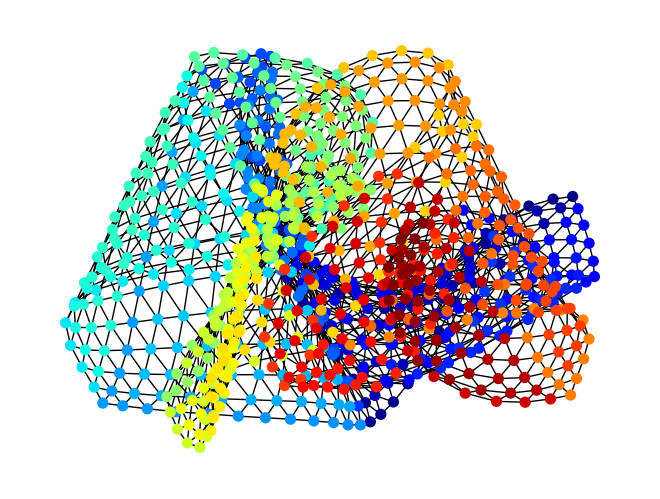
\includegraphics[width=\columnwidth]{jagmesh1_FR_50iter.png}
  \end{minipage}
  \begin{minipage}{0.49\hsize}
    \centering
    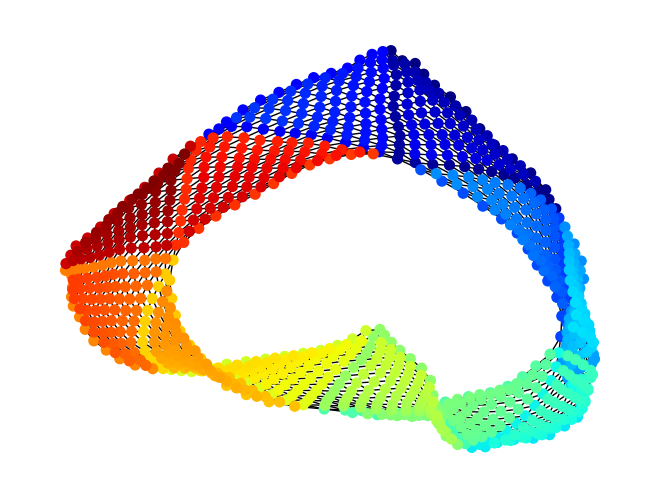
\includegraphics[width=\columnwidth]{jagmesh1_BFGS_50iter.png}
  \end{minipage}
  \caption{Comparison of the FR algorithm (left, NetworkX) and L-BFGS-B (right, my implementation) on the \texttt{jagmesh1} dataset.}
\end{figure}


\section{Preliminary}\label{sec:preliminary}

In this section, we define an optimization problem for FR algorithm.
Let $\bbR_+$ be a set of non-negative real numbers, $\bbR_{++}$ be a set of positive real numbers,
and $A = (a_{i,j}) \in \bbR_+^{n \times n}$ be an adjacency matrix of a undirected graph $G = (V, E)$.
Each vertex $v_i \in V$ is assigned a position $x_i \in \bbR^d$ and we define $x = (x_1, \dots, x_n) \in \bbR^{d \times n}$ as a matrix of positions.
For an optimal distance $k$, and a distance $d$ between two vertices $v_i$ and $v_j$, Fruchterman and Reingold defined the power of attraction $F_{i,j}^a: \bbR_{+} \to \bbR$ and the power of repulsion $F^r: \bbR_{++} \to \bbR$ as
\begin{equation*}
  F_{i,j}^a(d) \defeq \frac{a_{i,j} d^2}{k}, \quad F^r(d) \defeq -\frac{k^2}{d}.
\end{equation*}
The total energy for these powers $E_{i,j} : \bbR_{++} \to \bbR$, stress of the graph, is defined as
\begin{align*}
  E_{i,j}(d) & \defeq \int_{0}^{d} F_{i,j}^a(r) \dd{r} + \int_{\infty}^{d} F^r(r) \dd{r} \\
             & = \frac{a_{i,j} d^3}{3k} - k^2\log{d}.
\end{align*}
The energy function $E_{i,j}$ is convex for $a_{i,j} \in \bbR_{++}$ and minimized when $d = k/\sqrt[3]{a_{i,j}}$, but is not Lipschitz continuous.
Based on these energies, the optimization problem for FR algorithm is defined as
\begin{mini}
  {x \in \bbR^{d \times n}}
  {f(x) \defeq \sum_{i<j} E_{i,j}(d_{i,j})}
  {\label{eq:fr}}
  {}
\end{mini}
where $d_{i,j} = \norm{x_i - x_j}$ is the Euclidean distance.

In order to introduce the Random Subspace method, we define a function $f_i: \bbR^{d} \to \bbR$ for $1 \leq i \leq n$ as
\begin{equation*}
  f_i(x_i) \defeq \sum_{j \neq i} E_{i,j}(d_{i,j}).
\end{equation*}
The gradient and the Hessian of $f_i$ are
\begin{gather*}
  \nabla f_i(x_i) = \sum_{j \neq i} \qty(\frac{a_{i,j}d_{i,j}}{k} - \frac{k^2}{d_{i,j}^2}) (x_i-x_j), \\
  \nabla^2 f_i(x_i) = \sum_{j \neq i} \qty(\frac{a_{i,j}d_{i,j}}{k} - \frac{k^2}{d_{i,j}^2}) I_d +      \\
  \sum_{j \neq i} \qty(\frac{a_{i,j}}{k d_{i,j}} + \frac{2k^2}{d_{i,j}^4}) (x_i - x_j)(x_i - x_j)^\top.
\end{gather*}

As pointed out in~\cite{tunkelang1999numerical},
the FR algorithm is a gradient descent method for the energy function $f$.

\section{Algorithm} \label{sec:algorithm}

For $t \in [0,1)$, let define as
\begin{equation*}
  E_{i,j}^t(d) = \frac{a_{i,j} d^3}{3k} - \frac{k^2 d^{1-t} - 1}{1-t}.
\end{equation*}
Note that
\begin{equation*}
  \lim_{t \to 1} - \frac{k^2 d^{1-t} - 1}{1-t} = -k^2 \log{d}.
\end{equation*}
by \Lhopital's rule.

\begin{equation*}
  f_i^t(x_i) \defeq \sum_{j \neq i} E_{i,j}^t(d_{i,j}).
\end{equation*}
The gradient and the Hessian of $f_i$ are
\begin{gather*}
  \nabla f_i^t(x_i) = \sum_{j \neq i} \qty(\frac{a_{i,j}d_{i,j}}{k} - \frac{k^2}{d_{i,j}^{1+t}}) (x_i-x_j), \\
  \nabla^2 f_i^t(x_i) = \sum_{j \neq i} \qty(\frac{a_{i,j}d_{i,j}}{k} - \frac{k^2}{d_{i,j}^{1+t}}) I_d +      \\
  \sum_{j \neq i} \qty(\frac{a_{i,j}}{k d_{i,j}} + \frac{k^2(1+t)}{d_{i,j}^{3+t}}) (x_i - x_j)(x_i - x_j)^\top.
\end{gather*}

\subsection{Line Search}

We want to obtain
$
  \arg\min_{\alpha \geq 0} f_i(x + \alpha p).
$

In line search, we need to compute
\begin{align*}
  \pdv{\alpha} f_i(x+\alpha p)
   & = \pdv{\alpha} \sum_j E_{i,j}(\norm{(x_i + \alpha p) - (x_j + \alpha p)})                                                       \\
   & = \sum_j \pdv{\alpha} E_{i,j}(\norm{(x_i - x_j) + \alpha (p_i - p_j)})                                                          \\
   & = \sum_j \dv{d} E_{i,j}(d) \pdv{\alpha} \norm{(x_i - x_j) + \alpha (p_i - p_j)}                                                 \\
   & = \sum_j \dv{d} E_{i,j}(d) \frac{((x_i - x_j) + \alpha (p_i - p_j))^\top (p_i - p_j)}{\norm{(x_i - x_j) + \alpha (p_i - p_j)}}.
\end{align*}

\section{Experiment} \label{sec:experiment}

We used dataset from \cite{davis2011university} and MatrixMarket \cite{boisvertMatrixMarketWeb1997}.

\url{https://reference.wolfram.com/language/tutorial/GraphDrawingIntroduction.html}

\section{Conclusion} \label{sec:conclusion}

todo

\section*{Acknowledgment}

The author would like to thank ...

\ifthenelse{\boolean{isMain}}{
  \bibliographystyle{IEEEtran}
  \bibliography{FruchtermanReingoldByRandomSubspace}
}{}

\end{document}